\documentclass{article}
\usepackage{xcolor}
\definecolor{darkgreen}{rgb}{0.0, 0.5, 0.0}
\usepackage[utf8]{inputenc}
\usepackage{graphicx}
\usepackage{subcaption} % Use subcaption instead of subfigure
\usepackage{matlab-prettifier}
\usepackage{amsmath}

% Set equation numbering to section and subsection
%\renewcommand{\theequation}{\thesubsection.\arabic{equation}}
\makeatletter
\@addtoreset{equation}{subsection}
\makeatother
\usepackage{listings}
\usepackage{amssymb}
\usepackage{blindtext}
\usepackage{geometry}
\usepackage{graphicx}
\usepackage{float}
\usepackage{dirtytalk}
\usepackage{enumitem}
\usepackage{derivative}
\usepackage{biblatex}
\usepackage{enumitem}
\usepackage{pgfplots}
\usepackage{tikz}
\usepackage{svg}  % Enables SVG support
\usepackage{hyperref} % Enables hyperlinks
% No red boxes at hyperlinks
\hypersetup{
    colorlinks,
    linkcolor={blue},
    citecolor={blue},
    urlcolor={blue}
}

\lstset{
    language=Python,             % The language of the code
    basicstyle=\ttfamily\small,  % The font style for the code
    keywordstyle=\color{blue},   % Color of Python keywords
    stringstyle=\color{darkgreen},     % Color of strings
    commentstyle=\color{gray},  % Color of comments
    showstringspaces=false,      % Do not show spaces in strings
    frame=single,                % Frame around the code
    numbers=left,                % Line numbers on the left
    numberstyle=\tiny\color{gray},  % Style of the line numbers
    breaklines=true,             % Automatic line breaking
}%Imports biblatex package
 \geometry{
 a4paper,
 total={160mm,250mm},
 left=25mm,
 top=30mm,
 footskip =10mm,
 }

\title{Calculus Uge 3}
\author{Thomas Sejer Canham}
\date{\today} 
\setlength\parindent{0pt}

 \begin{document}

 \begin{titlepage}

    \maketitle

I denne uge skal vi arbejde med funktioner af to variable. I den sammenhæng skal vi arbejde med optimering af funktioner af to variable. Optimering af sådanne funktioner er foregår i bund og grunds på samme måde som optimering af funktioner af en variabel - dog med med nogle ekstra overvejelser angående hvilken type af kritisk punkt vi har med at gøre. Processen med at bestemme maksima og minima (eller saddelpunkter) for funktioner af to variable kan opdeles i følgende trin:

\begin{enumerate}
    \item Find de partielle afledte $f_x(x,y)$ og $f_y(x,y)$ af funktionen f(x,y) med hensyn til x og y.
    \item Løs ligningssystemet $f_x(x,y) = 0$ og $f_y(x,y) = 0$ for at finde de kritiske punkter $(x_0, y_0)$.
    \item Bestem typen af hvert kritisk punkt ved at beregne den anden afledte test. Dette indebærer at finde de andenordens partielle afledte $f_{xx}(x,y)$, $f_{yy}(x,y)$ og $f_{xy}(x,y)$.
    \item Beregn diskriminanten $D = f_{xx}(x_0,y_0) \cdot f_{yy}(x_0,y_0) - (f_{xy}(x_0,y_0))^2$ for hvert kritisk punkt.
    \item Brug diskriminanten til at bestemme typen af hvert kritisk punkt:
        \begin{itemize}
            \item Hvis $D > 0$ og $f_{xx}(x_0,y_0) > 0$, er $(x_0,y_0)$ et lokalt minimum.
            \item Hvis $D > 0$ og $f_{xx}(x_0,y_0) < 0$, er $(x_0,y_0)$ et lokalt maksimum.
            \item Hvis $D < 0$, er $(x_0,y_0)$ et saddelpunkt.
            \item Hvis $D = 0$, er testen ubestemt.
        \end{itemize}
\end{enumerate}
Det er værd at bemærke, at når vi differentierer funktioner af to variable, anses andre variable som konstante fra synspunktet af den variable, vi differentierer med hensyn til. For eksempel, når vi differentierer $f(x,y)$ med hensyn til $x$, betragtes $y$ som en konstant, og omvendt.\vspace{1em}

\emph{Ugens hint er at hvis i følger overstående trin til punkt og prikke, vil i kunne løse ugens afleverings opgave relativt problemfrit.} \vspace{1em}

Til den interesserede, er dette et område der er meget anvendt i den virkelige verden. Det kan generaliseres til funktioner af $n$ variable, og er grundlaget for optimering i maskinlæring, økonomi, fysik og mange andre områder. Generaliseringen kræver dog linær algebra og vektorkalkulus, men de grundlæggende principper forbliver de samme. Givet en funktion $f(x_1, x_2, \ldots, x_n)$, kan vi finde kritiske punkter ved at finde gradienten $\nabla f = \left( \frac{\partial f}{\partial x_1}, \frac{\partial f}{\partial x_2}, \ldots, \frac{\partial f}{\partial x_n} \right)$ og sætte den lig med nulvektoren. Derefter kan vi bruge den anden afledte test, som involverer Hesse-matricen

$$H = \begin{pmatrix}
    f_{x_1x_1} & f_{x_1x_2} & \cdots & f_{x_1x_n} \\
    f_{x_2x_1} & f_{x_2x_2} & \cdots & f_{x_2x_n} \\
    \vdots & \vdots & \ddots & \vdots \\
    f_{x_nx_1} & f_{x_nx_2} & \cdots & f_{x_nx_n}
\end{pmatrix}$$
Som kan have forskellige egenskaber (definithed) afhængigt af de kritiske punkter, hvilket giver os information om typen af hvert kritisk punkt. Det bør dog bemærkes, at det er kun meget specifikke tilfælde, hvor vi kan være sikre på at vi har fundet et globalt maksimum eller minimum. I de fleste tilfælde vil vi kun kunne bestemme lokale ekstrema uden yderligere information om funktionens adfærd i hele dens domæne.


\end{titlepage}

\section*{Eksempel}

    Vi betragter funktionen

\[
f(x,y)=4x+6y-x^2-xy-y^2.
\]

Vi vil bestemme funktionens maksimum ved hjælp af de partielle
afledte og den anden afledte test.

\begin{figure}[H]    

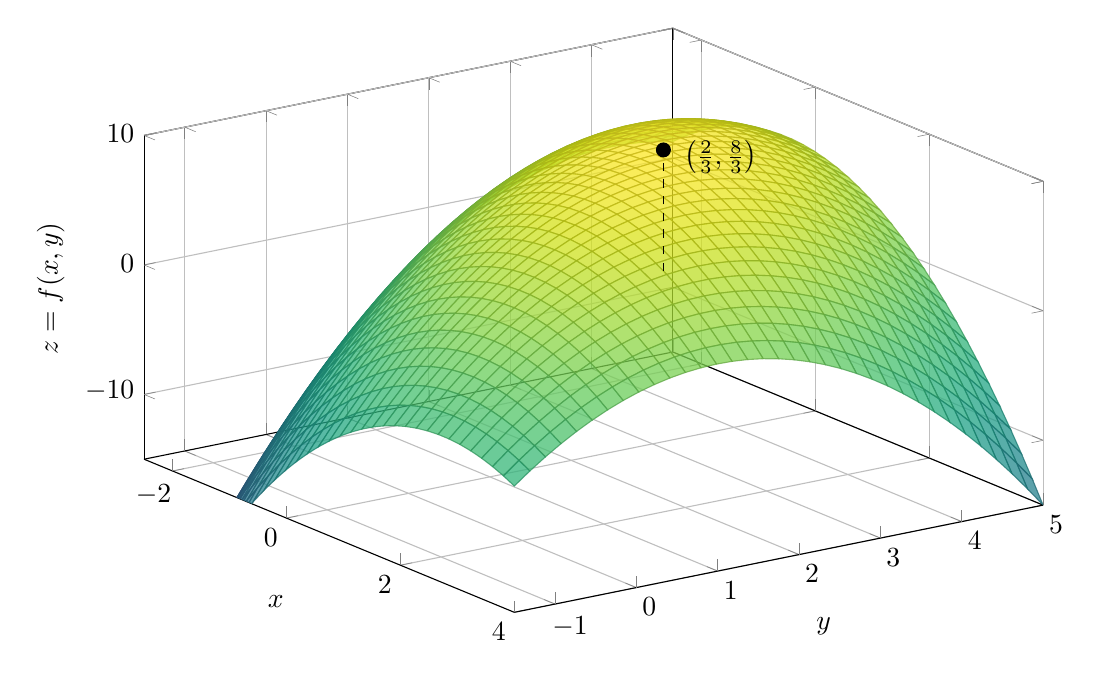
\begin{tikzpicture}
\begin{axis}[
    width=13cm,
    height=9cm,
    view={55}{30},
    xlabel={$x$},
    ylabel={$y$},
    zlabel={$z=f(x,y)$},
    xmin=-2.5, xmax=4,
    ymin=-1.5, ymax=5,
    zmin=-15, zmax=10,
    grid=major,
    colormap/viridis,
]

% Grafen
\addplot3[
    surf,
    domain=-2.5:4,
    y domain=-1.5:5,
    samples=35,
    opacity=0.75,
]
{4*x + 6*y - x^2 - x*y - y^2};

% Maksimumspunkt
\addplot3[
    only marks,
    mark=*,
    mark size=2.5pt
]
coordinates {(2/3,8/3,28/3)};

% Lodret linje til maksimumspunktet
\addplot3[
    dashed
]
coordinates {(2/3,8/3,0) (2/3,8/3,28/3)};

% Label
\node at (axis cs:1.2,3.0,9.3)
{$\left(\frac23,\frac83\right)$};

\end{axis}

\end{tikzpicture}
\caption{Illustration af eksempelproblemet}
    \label{fig:optimering}
\end{figure}

\begin{enumerate}

    \item \textbf{Find de partielle afledte}

    Vi bestemmer de partielle afledte med hensyn til $x$ og $y$:

    \[
    f_x(x,y)=4-2x-y
    \]

    og

    \[
    f_y(x,y)=6-x-2y.
    \]

    \item \textbf{Find de kritiske punkter}

    De kritiske punkter findes ved at løse ligningssystemet

    \[
    \begin{cases}
    4-2x-y=0,\\
    6-x-2y=0.
    \end{cases}
    \]

    Vi omskriver den første ligning:

    \[
    2x+y=4.
    \]

    Den anden ligning giver

    \[
    x+2y=6.
    \]

    Vi har derfor systemet

    \[
    \begin{cases}
    2x+y=4,\\
    x+2y=6.
    \end{cases}
    \]

    Fra den første ligning får vi

    \[
    y=4-2x.
    \]

    Dette indsættes i den anden ligning:

    \[
    x+2(4-2x)=6.
    \]

    Dermed får vi

    \[
    x+8-4x=6,
    \]

    og derfor

    \[
    -3x=-2,
    \]

    så

    \[
    x=\frac{2}{3}.
    \]

    Vi finder nu $y$:

    \[
    y=4-2\left(\frac{2}{3}\right)
    =4-\frac{4}{3}
    =\frac{8}{3}.
    \]

    Det kritiske punkt er altså

    \[
    \boxed{\left(\frac{2}{3},\frac{8}{3}\right)}.
    \]

    \item \textbf{Bestem de andenordens partielle afledte}

    De andenordens partielle afledte er

    \[
    f_{xx}(x,y)=-2,
    \]

    \[
    f_{yy}(x,y)=-2,
    \]

    og

    \[
    f_{xy}(x,y)=-1.
    \]

    \item \textbf{Beregn diskriminanten}

    Diskriminanten er

    \[
    D=
    f_{xx}(x_0,y_0)f_{yy}(x_0,y_0)
    -
    \left(f_{xy}(x_0,y_0)\right)^2.
    \]

    Vi får derfor

    \[
    D=(-2)(-2)-(-1)^2
    =4-1
    =3.
    \]

    Altså er

    \[
    D>0.
    \]

    \item \textbf{Bestem typen af det kritiske punkt}

    Vi har

    \[
    D>0
    \]

    og

    \[
    f_{xx}\left(\frac23,\frac83\right)=-2<0.
    \]

    Derfor er

    \[
    \boxed{\left(\frac23,\frac83\right)}
    \]

    et lokalt maksimum. Funktionsværdien i punktet er

    \[
    f\left(\frac23,\frac83\right)
    =
    4\left(\frac23\right)
    +6\left(\frac83\right)
    -\left(\frac23\right)^2
    -\left(\frac23\right)\left(\frac83\right)
    -\left(\frac83\right)^2.
    \]

    Dette giver

    \[
    f\left(\frac23,\frac83\right)
    =\frac{28}{3}.
    \]


\end{enumerate}


\end{document}
